\documentclass[11pt]{extarticle}
\usepackage{manualdoprofessor}
\usepackage{fichatecnica}
\usepackage{lipsum,media9}
\usepackage[justification=raggedright]{caption}
\usepackage[one]{bncc}
\usepackage[acorde]{../edlab}
\usepackage{marginnote}
\usepackage{pdfpages}
\usepackage[printwatermark]{xwatermark}
% \newwatermark[pagex=2]{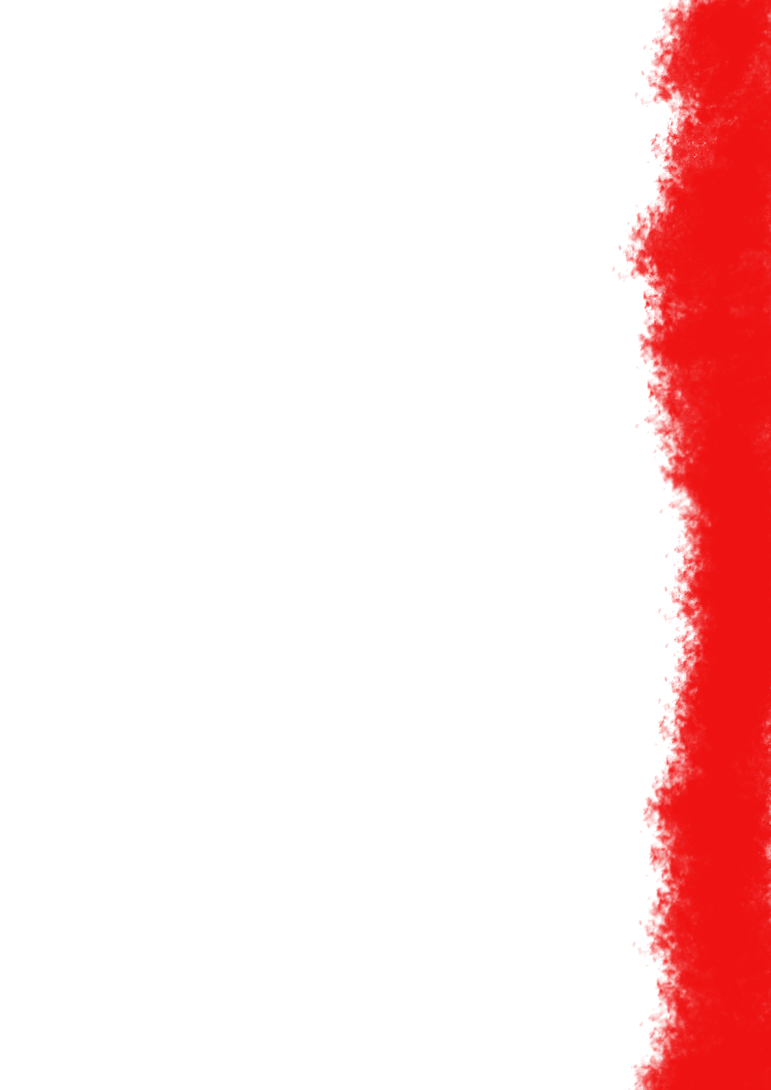
\includegraphics[scale=3.3]{watermarks/test-a.png}}	% página específica
% %\newwatermark[oddpages]{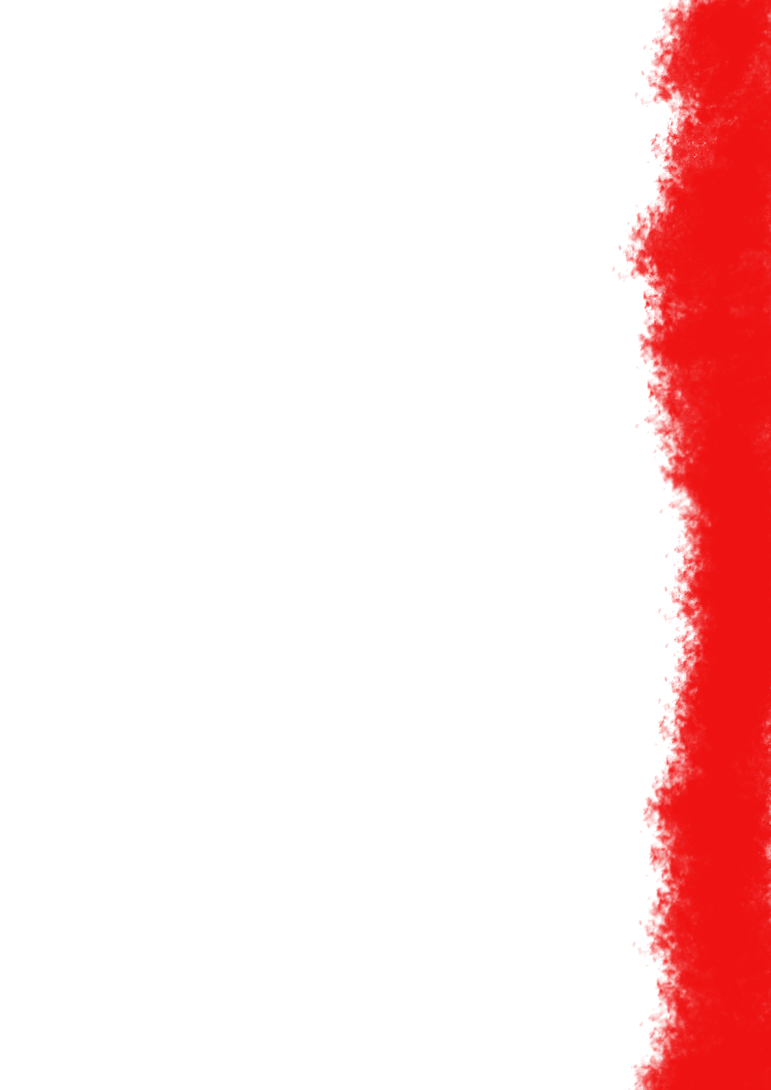
\includegraphics{watermarks/test-a.png}}			% páginas ímpars
% %\newwatermark[evenpages]{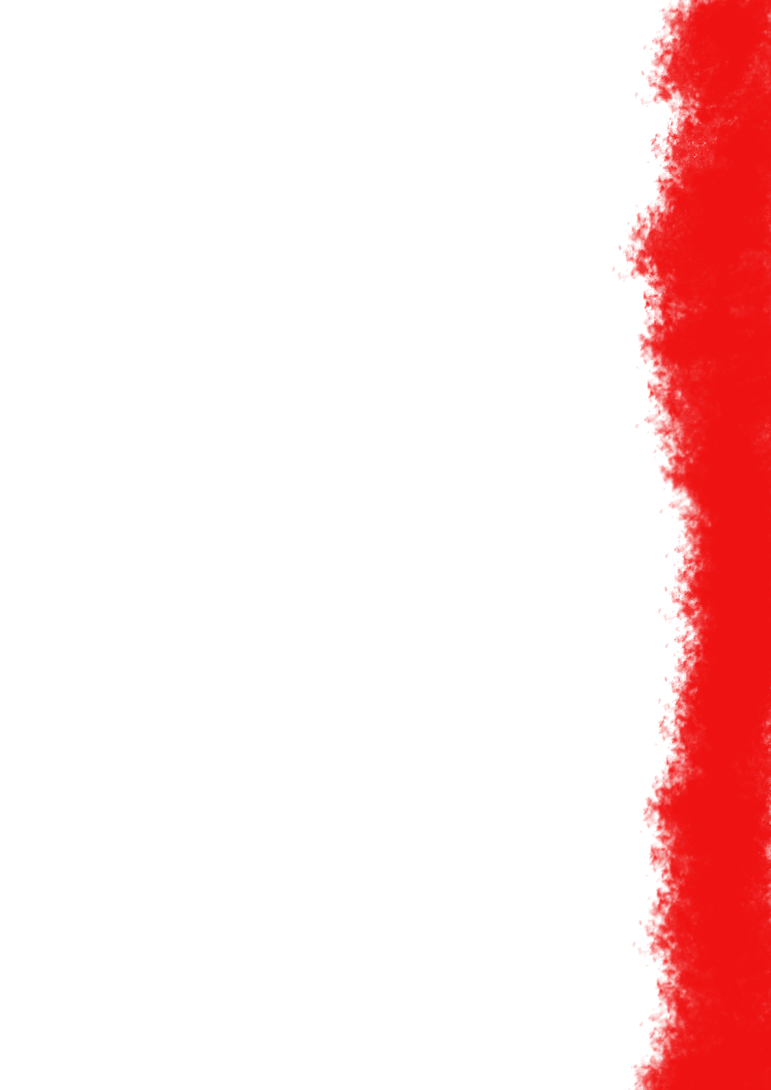
\includegraphics{watermarks/test-a.png}}			% págimas pares
% \newwatermark[allpages]{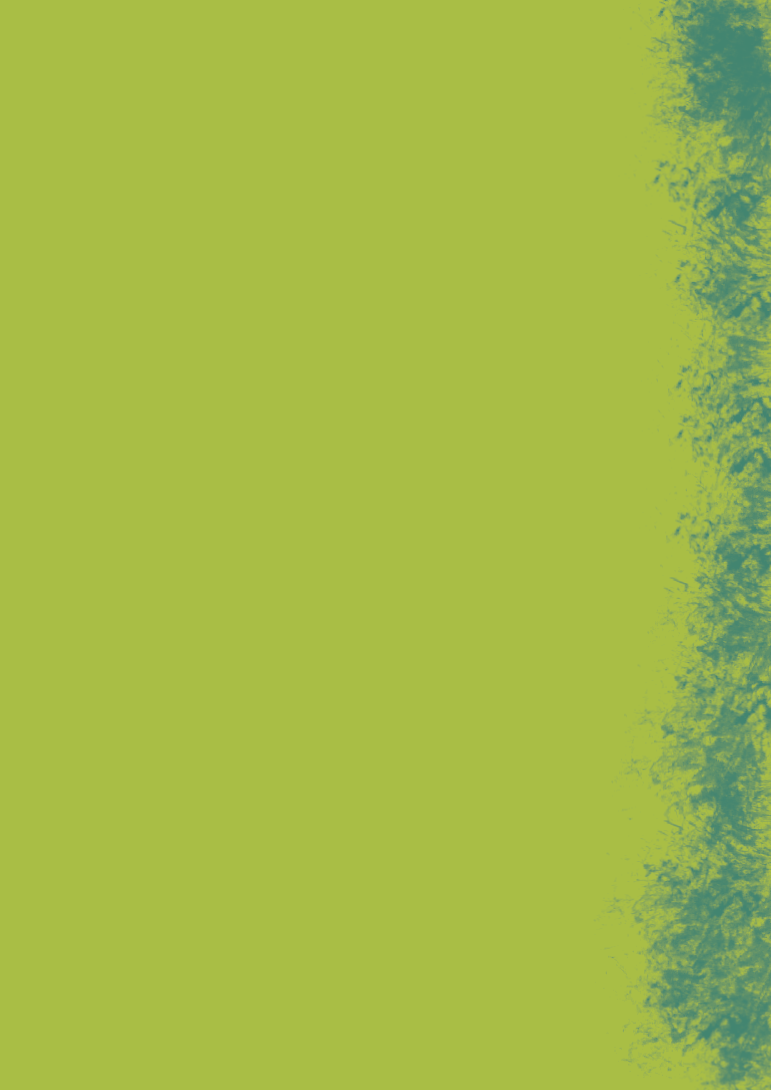
\includegraphics[scale=3.3]{watermarks/test-b.png}}

% \pagecolor{cyan!0!magenta!10!yellow!28!black!28!}

\newcommand{\AutorLivro}{Antonio Prata}
\newcommand{\TituloLivro}{Esconde-Esconde}
\newcommand{\Genero}{Poesia}
%\newcommand{\imagemCapa}{./images/PNLD0001-01.png}
\newcommand{\issnppub}{978-65-99441-24-0}
\newcommand{\issnepub}{978-65-99441-27-1}
% \newcommand{\fichacatalografica}{PNLD0001-00.png}
\newcommand{\colaborador}{Gabriela Karam}

\begin{document}

\title{\TituloLivro}
\author{\AutorLivro}
\def\authornotes{\colaborador}

\date{}
\maketitle

%\begin{abstract}\addcontentsline{toc}{section}{Carta ao professor}
%\pagebreak

\tableofcontents


\begin{abstract}

Caras e caros educadores,

O presente manual tem como objetivo oferecer uma orientação sobre a obra \textit{Esconde-Esconde}. A partir deste material, você poderá incentivar os estudantes à leitura e proporcionar-lhes um conteúdo enriquecedor. Apresentamos aqui sugestões de atividades a serem realizadas antes, durante e após a leitura do livro, com propostas que buscam introduzir os gêneros literários e aprofundar as discussões trazidas pelas obras. Você encontrará informações sobre o autor, sobre o gênero e sobre os temas trabalhados ao longo do livro. Ao fim do manual, você encontrará também sugestões de livros, artigos e sites selecionados para enriquecer a sua experiência de leitura e, consequentemente, a de seus estudantes.

\Image{Ilustração do livro (Imagem do livro, pag. 6)}{PNLD2023-035-02.png}

O livro é uma imersão no mundo das palavras, suas partes e seus significados. O autor propõe a seguinte brincadeira: procurar palavras dentro de palavras.

\textit{Já reparou que, às vezes, dentro de uma palavra, outra palavra se esconde? Aqui, ó, do bumbum do esc eis que surge um onde.}

Esse é o mote para o autor tratar de maneira lúdica um tema clássico da linguística de Ferdinand de Saussure: a arbitrariedade do signo linguístico, ou seja, o fato de que a relação entre o som (significante) e o sentido (significado) de uma palavra é arbitrária. A formação de palavras é um dos temas mais importantes para os estudantes do Ensino Fundamental como um todo, visto que o entendimento do português depende do começo: conhecer usos e significados dos radicais das palavras e dos afixos que são adicionados a eles. 

Nossa proposta é aceitar o convite do autor e propor a utilização de jogos para um aprofundamento da leitura mais lúdico e divertido. Contamos com vocês para mergulharmos juntos nessa história cheia de brincadeiras com palavras e rimas espirituosas. 

Esperamos que as atividades sugeridas e o material indicado sejam proveitosos em sala de aula! 

\end{abstract}

\section{Sobre o livro}

\textit{Esconde-Esconde} é um livro escrito por Antonio Prata e ilustrado por Talita Hoffmann, a mesma dupla dos infantis \textit{Jacaré, não!} e \textit{A menina que morava no chuveiro}. 

O livro parte do pressuposto de que algumas palavras “escondem” outras. É uma mina inesgotável de brincadeiras com as palavras e de ilustraçõs criativas, curiosas e engraçadas. A partir da proposta inicial do autor e da ilustradora, o professor pode propor atividades para explorar palavras e partes de palavras, tanto do ponto de vista da escrita, quanto do som: dentro da palavra \textit{esconde} pode-se encontrar a palavra \textit{onde}. As últimas duas páginas do livro já sugerem: o aluno-leitor deve pegar a lista de palavras sugeridas pelo autor e criar seus próprios textos.

Além disso, vale ressaltar que as ilustrações de Hoffmann são muito certeiras por conta das cores e detêm uma identificação muito clara com as crianças e os pré-adolescentes. A genialidade da obra está na fusão entre uma narrativa que gera muito interesse e que, ao mesmo tempo, tem rimas e jogos de palavras muito ricos para o entendimento da língua portuguesa. Ao longo desse manual, sugestões para atividades e algumas referências serão compartilhadas para que a leitura e o trabalho com o livro sejam mais proveitosos e aprofundados. Usando e abusando de formas lúdicas para se contar uma história, verificamos no livro a presença de respostas para perguntas que as crianças costumam fazer, como por exemplo: será que um pássaro voa daqui até a Argentina se quiser? Com maestria, autor e ilustradora proporcionam uma série de questionamentos para as crianças, além de aflorar muito a criatividade dos pequenos.

\section{Sobre o autor}

Antonio Prata, que é  filho dos também escritores Mário Prata e Marta Góes, já publicou vários livros e é roteirista e autor contratado pela Rede Globo, onde colaborou em várias novelas, entre elas \textit{Bang Bang}, de seu pai Mário Prata e Carlos Lombardi, e a célebre \textit{Avenida Brasil}. Em 2015 escreveu o piloto da série \textit{Os Experientes}, dirigido por Kiko e Fernando Meirelles, que venceu o prêmio APCA de melhor série de televisão e foi finalista do Emmy Awards. Em 2012, foi incluído na edição brasileira da revista Granta como um dos vinte melhores escritores nacionais com menos de 40 anos. Desde 2010 também escreve aos domingos no caderno da Folha de São Paulo, vem se aventurando já há um tempo no universo infantil. E agora, em \textit{Esconde Esconde}, parte para uma empreitada linguística: com um texto bem sacado e ilustrações super imaginativas, o livro convida, com muito humor, crianças e adultos a pensarem e tomarem consciência da composição das palavras em português.

\section{Sobre o gênero}

\paragraph{O gênero} O gênero deste livro é o da \textit{poesia}. 

\paragraph{Descrição} Um dos meios mais expressivos de comunicação e inovação da linguagem, a poesia é uma das mais antigas formas de arte literária, anterior até mesmo à escrita, pois existe desde a tradição oral. Ela combina palavras, significados, sonoridades, ritmos e, muitas vezes, também imagens para permitir uma experiência estética. A linguagem poética é condensada e emotiva e busca trabalhar a língua de forma que o leitor experimente as palavras de uma forma nova. Na maior parte das vezes, a poesia é dividida em versos que, juntos, são chamados de estrofes. O ponto de vista do autor e sua visão pessoal do mundo estão muito presentes nesse tipo de texto e, justamente por essa particularidade, a experiência da leitura de uma poesia é extremamente individual e subjetiva.

\paragraph{Interação} Esse gênero é um grande aliado na formação do leitor. O olhar da criança para o mundo é, em essência, um olhar poético, calcado na curiosidade pelo mundo. A poesia é a forma perfeita de valorizar esse olhar e incentivar que a criança brinque com as palavras, observe os sons e experimente novos ritmos. Por sua liberdade e criatividade, a poesia tem potencial para estabelecer um diálogo único com os pequenos leitores. A presença de fantasias, imagens, repetição e símbolos permite uma maior identificação, pois a criança ainda está construindo seu mundo interior e experimenta a vida de forma diferente do adulto. 

\section{Proposta de Atividades}
\subsection{Pré Leitura}
\subsubsection{Atividade 1}

\BNCC{EF03LP10}% Reconhecer prefixos e sufixos produtivos na formação de palavras derivadas de substantivos, de adjetivos e de verbos, utilizando-os para compreender palavras e para formar novas palavras.


\paragraph{Tema} As palavras: som e sentido. 

\paragraph{Conteúdo} Jogos com as palavras. 

\paragraph{Objetivo} Estimular o contato com as palavras, de modo a apreender-lhes a estrutura e o sentido. 

\paragraph{Justificativa} Para os estudantes, os jogos com as palavras despertam questionamentos que levam ao tema do livro: o sentido, os sons e a estrutura das palavras.   

Antes de mergulhar no universo da obra \textit{Esconde Esconde}, o educador pode estimular os alunos a explorarem as palavras de uma forma geral. Para isso, antes de mais nada, pergunte e debata com os estudantes sobre a formação de palavras através das letras e dos sons. Logo em seguida, proponha um caça palavras entre eles e, com isso, acabará provocando uma intimidade com as letras e os processos de formação de palavras. 

\paragraph{Metodologia} Antes de mergulhar no universo da obra \textit{Esconde Esconde}, o educador pode estimular os alunos a explorarem as palavras de uma forma geral. Para isso, antes de mais nada, pergunte e debata com os estudantes sobre a formação de palavras através das letras e dos sons. Logo em seguida, proponha um caça palavras entre eles e, com isso, acabará provocando uma intimidade com as letras e a formação de palavras. 

Outro jogo muito interessante e que também provoca algo bastante parecido com o anterior a respeito da desenvoltura com a nossa língua é a Forca. 

Algumas dicas para que esse jogo fique divertido e estimulante para os estudantes: 


\begin{itemize}
\item Divida a turma em grupos de cinco estudantes cada;
\item Escolha palavras aleatórias dentro do universo dos estudantes para não desestimular a turma;
\item Coloque apenas as linhas de cada letra com a formação da palavra no quadro escolar; 
\item Inicie o jogo para a descoberta da palavra através das letras escolhidas. Organize os estudantes de modo que a turma inteira participe;
\item Aguce a perspicácia deles, desperte o interesse pela palavra e, conforme o jogo for fluindo, escolha palavras mais difíceis para incentivá-los cada vez mais.

\end{itemize}

Uma vez concluídas as rodadas, aproveite as palavras trabalhadas para trazer o tema de formação de palavras. Com a participação dos estudantes, identifique as partes de palavras e suas funções: mostre as contribuições semânticas dos prefixos, a mudança de classe gramatical trazida pelos sufixos e a função do radical. É um bom momento para que o professor traga à tona os tipos de formação: por composição ou por derivação. Depois te trazer a teoria, é interessante colocá-los para praticar. E um jogo muito interessante para isso é o Stop:

\begin{itemize}
\item Solicite que todos os estudantes tenham papel e caneta nas mãos;
\item Defina as categorias de acordo com a idade da turma. Por exemplo: Nome, Fruta, Cor, Cidade;
\item Escolha uma letra para que todos comecem a preencher;
\item A primeira pessoa que terminar de preencher tudo primeiro grita Stop e todo mundo para de escrever;
\end{itemize}

Aproveite para debater depois dos jogos sobre as dificuldades e as facilidades dentro das atividades propostas, perguntando a eles quais processos de formação de palavras apareceram ao longo das brincadeiras. Por fim, forneça aos estudantes subsídios para pensar sobre as palavras e como elas nos ajudam em uma comunicação mais clara com nós mesmos e com o mundo, fortalecendo, assim, não só a nossa autoestima, como a noção de cidadania.

\subsubsection{Atividade 2}

\BNCC{EF15AR01}% Identificar e apreciar formas distintas das artes visuais tradicionais e contemporâneas, cultivando a percepção, o imaginário, a capacidade de simbolizar e o repertório imagético.
\BNCC{EF15AR04}% Experimentar diferentes formas de expressão artística (desenho, pintura, colagem, quadrinhos, dobradura, escultura, modelagem, instalação, vídeo, fotografia etc.), fazendo uso sustentável de materiais, instrumentos, recursos e técnicas convencionais e não convencionais.

Quando mergulhamos no mundo das palavras, um universo infinito de imagens surge nas nossas cabeças, provocando signos que fazem com que elas digam a que vieram. No livro \textit{Esconde-Esconde}, os desenhos que ilustram o texto fazem parte integrante da história. A pessoa que executa uma ilustração de um livro, é uma das personagens principais na literatura, em especial na literatura para crianças. É ela quem dá imagem, cor e formas à ideia do texto, ou até mesmo conta a história por meio das ilustrações. 

Portanto, essa segunda atividade tem como objetivo desenvolver o aprofundamento do contato da palavra através de imagens. Selecione algumas das palavras usadas na atividade anterior e estimule a criação de desenhos ou colagens relacionadas a elas. Atenção à sustentabilidade dos materiais usados. Aproveite para apresentar algumas ilustrações de livros diversos. Não se limite só às ilustrações mais concretas, provoque um pouco mais e mostre algumas mais abstratas para que os estudantes ampliem sua observação de leitura de imagens. Acreditamos que depois dessas atividades, os estudantes já estarão prontos para uma leitura comprometida e ao mesmo tempo divertida. 

\paragraph{Tempo Estimado} Quatro aulas de 50 minutos. 

PNLD2023-035-09.

\section{Leitura}

\BNCC{EF02LP26}% Ler e compreender, com certa autonomia, textos literários, de gêneros variados, desenvolvendo o gosto pela leitura.
\BNCC{EF15LP04}% Identificar o efeito de sentido produzido pelo uso de recursos expressivos gráfico-visuais em textos multissemióticos.

\paragraph{Tema} Leitura e compreensão de \textit{Esconde-Esconde}.

\paragraph{Conteúdo} Estrutura de de \textit{Esconde-Esconde}.  

\paragraph{Objetivo} Ler e compreender o texto de \textit{Esconde-Esconde} e seus pressupostos. Promover o gosto pelos livros e pela leitura, estimular o desenvolvimento da linguagem, enriquecer o vocabulário e aumentar o conhecimento a respeito das palavras e suas partes.   

\paragraph{Justificativa} O professor tem grande influência na formação de leitores, especialmente quando se trata de compreender e analisar as palavras, para ampliar o repertório cultural dos alunos. É preciso fazer a mediação entre a obra, sua linguagem, suas estruturas, seus pressupostos e os estudantes, de preferência estabelecendo uma relação fundamentada no prazer, na identificação e na liberdade de interpretação. Eis o nosso desafio: ler com os alunos, apresentando as passagens decisivas de um texto, explicando por que elas chamam a atenção e  ouvindo as impressões dos estudantes a respeito de tudo isso.  

Antes de iniciar a leitura, coloque as cadeiras em roda para que os estudantes possam ver uns aos outros e obter aquela sensação de histórias contadas em volta da fogueira. Como esse livro tem uma presença muito forte das ilustrações, que estão lado a lado com a narrativa, sugerimos que a leitura seja compartilhada e que, a cada página, a pessoa que estiver lendo apresente para a turma as ilustrações de forma que os desenhos possam ser vistos e apreciados por todo mundo. 

Outra sugestão é que o professor realize uma primeira leitura integral para apresentar a narrativa e elucidar possíveis dúvidas, como algumas palavras que podem apresentar maior dificuldade de compreensão. Sanar as questões das palavras dentro de outras e como as ilustrações vão colocando essas palavras num lugar lúdico e fantástico. Em seguida, pode-se fazer uma demonstração apenas das ilustrações para a descoberta da riqueza de detalhes que acompanham cada página. Essa forma de leitura acompanhada entre o professor e a turma facilita a apreensão da narrativa e do estudo das palavras em questão.

Incentive que os estudantes interajam com a obra, trazendo para seus gostos e impressões. Pode-se fazer perguntas como:

\begin{itemize}
\item De qual estrofe vocês mais gostaram?
\item Algumas dessas palavras vocês acharam difícil de identificar dentro da outra? Quais?
\item Qual parte vocês acharam mais interessante? Por quê?
\item Qual ilustração vocês tiveram mais dificuldade de entender? Por quê?
\item Quais foram os processos de formação de palavras mais recorrentes?
\end{itemize}

Dessa forma, estimula-se a apreensão do enredo, do conteúdo da formação de palavras e das ilustrações que estão completamente em consonância com a proposta do livro.

\paragraph{Tempo Estimado} Duas aulas de 50 minutos. 

\section{Pós-leitura}

\BNCC{EF15LP18}% Relacionar texto com ilustrações e outros recursos gráficos.
\BNCC{EF12LP05}% Planejar e produzir, em colaboração com os colegas e com a ajuda do professor, (re)contagens de histórias, poemas e outros textos versificados (letras de canção, quadrinhas, cordel), poemas visuais, tiras e histórias em quadrinhos, dentre outros gêneros do campo artístico-literário, considerando a situação comunicativa e a finalidade do texto.

\paragraph{Tema} Vocabulário. 

\paragraph{Conteúdo} Estrutura e significado das palavras.

\paragraph{Objetivo} Ampliar o vocabulário e desenvolver exercícios de escrita.

\paragraph{Justificativa} Enquanto as atividades de leitura, compreensão e análise caracterizam-se pelas primeiras aproximações do texto, seguidas de atividades de descrição de suas características, a prática de redação abre espaço para que os estudantes criem suas próprias narrativas. Além disso, os jogos com as palavras também servem para ampliar o vocabulário. 

\paragraph{Metodologia} Nas páginas finais de \textit{Esconde-Esconde}, o autor propõe uma atividade que envolve outras novas palavras para que os leitores brinquem da mesma forma apresentada no livro. 

Divida a turma em grupos e, utilizando o quadro, escreva as palavras propostas pelo autor. Em seguida, para que todo mundo participe, escolha uma palavra e peça para que um grupo descubra quais palavras se escondem nela e circule com uma caneta ou giz colorido para enfatizar bem a palavra encontrada, e assim sucessivamente até as palavras acabarem. Peça que identifiquem se houver formação de palavras por composição ou derivação. Ao final desta atividade, proponha que os mesmos grupos tentem encontrar outras palavras que tenham palavras escondidas. Refaça o exercício anterior, desta vez com as palavras que os grupos propuseram. Esse exercício estimula a busca por palavras novas e o aumento do vocabulário, assim como a proximidade com a língua portuguesa.

Uma outra atividade que poderá ser desenvolvida é a criação de um poema como o do livro, utilizando a nova lista de palavras que acabou de ser criada. Se for necessário, leia junto com os estudantes novamente o livro para ter novas ideias. Incentive e aguce a imaginação deles apresentando rimas e trocadilhos possíveis com as palavras propostas. Lembre que é importante que o professor acompanhe o processo da escrita, tirando dúvidas e ajudando em possíveis dificuldades. Relembre que eles podem usar ilustrações para ajudar a contar essa história e estimule a realização de desenhos que comuniquem conforme a preferência de cada grupo.

Dessa forma, além de desenvolver a prática da escrita, o aluno consegue organizar melhor suas impressões da obra. Pode, assim, equilibrar os aspectos que mais lhe agradaram durante a leitura, bem como o que apreendeu a partir dos debates e dos exercícios desenvolvidos em sala de aula. Como forma de orientar e estimular os estudantes, o professor pode relembrar as atividades em torno da tarefa de pré-leitura, na qual diversas palavras foram reveladas e como a construção de uma narrativa através de palavras pode ser rica e atrativa para quem lê.

\section{Sugestões de referências complementares}

\subsection{Livros} 

\begin{itemize}
\item \textsc{rylant}, Cynthia. \textit{A velhinha que dava nome às coisas}. São Paulo: Brinque-Book, 2002.

Livro que conta a história de uma velhinha que já não tinha nenhum amigo, pois todos eles haviam morrido. Por isso, ela começa a dar nome às coisas que durariam mais que ela: sua casa, seu carro, sua poltrona, até o dia em que um cachorrinho apare no seu portão.

\item \textsc{bandeira}, Pedro. \textit{Mais respeito, eu sou criança!} São Paulo: Moderna, 2009.

Livro sobre a necessidade de as crianças expressarem seus sentimentos e suas memórias por meio da via literária.

\end{itemize}

\section{Bibliografia comentada}
\subsection{Livros}

\begin{itemize}
\item \textsc{brasil}. Ministério da Educação. \textit{Base Nacional Comum Curricular}. Brasília, 2018.

Consultar a \textsc{bncc} é essencial para criar atividades para a turma. Além de especificar quais habilidades precisam ser desenvolvidas em cada ano, é fonte de informações sobre o processo de aprendizagem infantil. 

\item \textsc{meireles}, Cecília. \textit{Ou isto ou aquilo}. São Paulo: Global Editora, 2012.

O tema do livro é que a vida é feita de escolhas que muitas vezes são difíceis de resolver, o cotidiano marcado pela dúvida e pela dificuldade de decisão, de forma poética e brincando com os pronomes demonstrativos.

\item \textsc{bojunga}, Lygia. \textit{A bolsa amarela}. São Paulo: Casa Lygia Bojunga, 2013.

A bolsa amarela é o romance de uma menina que entra em conflito consigo mesma e com a família ao reprimir três grandes vontades que ela esconde numa bolsa amarela.

\item \textsc{porto}, Cristina. \textit{O diário escondido da Serafina}. São Paulo: Ática, 2021.

Livro que traz a história de Serafina, uma menina que tem seu diário e deixa escondido na casa de seu avô.

\item \textsc{coelho}, Nelly Novaes. \textit{Literatura infantil, teoria, análise, didática}. 1ª ed. São Paulo: Moderna, 2000.

Livro que fala sobre os espaços da literatura infantil na contemporaneidade e a importância de as crianças estarem ligadas ao seu imaginário pela via literária.

\item \textsc{paixão}, Fernando. \textit{Poesia a gente inventa}. São Paulo: FTD Educação, 2019.

Livro que traz cinco poemas para crianças, vinculados às ilustrações.

\end{itemize}

\subsection{\textit{Sites}}

\begin{itemize}
\item Artigo \href{https://siteantigo.portaleducacao.com.br/conteudo/artigos/educacao/a-importancia-da-leitura-dos-contos-de-fadas-na-educacao-infantil/30151}{``A Importância da Leitura dos Contos de Fadas na Educação Infantil''}, por Ana Maria da Silva.

Artigo sobre a importância da construção do imaginário pela via da literatura para as crianças, trazendo elementos que analisam o mundo pós-moderno e os espaços que a literatura para crianças, principalmente os contos, devem ter.

\item Reportagem \href{http://www.multirio.rj.gov.br/index.php/leia/reportagens-artigos/reportagens/3059-biografias-para-criancas-a-palavra-de-quem-faz}{``Biografia para crianças, a palavra de quem faz''}.

Reportagem sobre como contar histórias biográficas para crianças.

\end{itemize}

\subsection{\textit{Filmes}}

\begin{itemize}
\item \textit{O menino maluquinho}. Dirigido por Helvécio Ratton, 1995.

No final dos anos 1960, o Menino Maluquinho é um garoto normal, feliz e bem cuidado por sua família que, enquanto aproveita a infância brincando na rua com a turma, observa o mundo que o cerca e aprende a lidar com a vida.

\item \textit{Meu pé de laranja lima}. Dirigido por Marcos Bernstein, 2013.

Zezé é um garoto de oito anos que, apesar de levado, tem um bom coração. Ele leva uma vida bem modesta, devido ao fato de seu pai estar desempregado há bastante tempo, e tem o costume de ter longas conversas com um pé de laranja lima que fica no quintal de sua casa. Até que, um dia, conhece Portuga, um senhor que passa a ajudá-lo e logo se torna seu melhor amigo.


\end{itemize}
\end{document} 
